% !TEX program = xelatex
% =====================================================================
%  LUỒNG NGHIỆP VỤ — Hệ thống quản lý minh chứng KĐCLGD (kdcl-v2)
%  Format & font: theo deck Hiệu trưởng DAU (maroon/gold/navy, Noto Sans)
%  Tác giả: TS. Đỗ Phúc Hảo, Giám đốc Trung tâm CAIRA
%  Compile: xelatex luong-kdcl.tex  (chạy 2 lần cho header/footer/refs)
% =====================================================================
\documentclass[aspectratio=169, 11pt]{beamer}

% ---------- Fonts & Vietnamese ----------------------------------------
\usepackage{fontspec}
\setsansfont{Noto Sans}[Ligatures=TeX, BoldFont={Noto Sans Bold}, ItalicFont={Noto Sans Italic}]
\setmainfont{Noto Sans}[Ligatures=TeX]
\setmonofont{Noto Sans Mono}[Scale=0.86]
\usepackage{polyglossia}
\setdefaultlanguage{vietnamese}
\setotherlanguage{english}
\usepackage{newunicodechar}
\newunicodechar{→}{\ensuremath{\rightarrow}}
\newunicodechar{←}{\ensuremath{\leftarrow}}
\newunicodechar{↑}{\ensuremath{\uparrow}}
\newunicodechar{↓}{\ensuremath{\downarrow}}
\newunicodechar{≥}{\ensuremath{\geq}}
\newunicodechar{≤}{\ensuremath{\leq}}
\newunicodechar{·}{\ensuremath{\cdot}}
\newunicodechar{×}{\ensuremath{\times}}

% ---------- Palette chuẩn trường (DAU) --------------------------------
\usepackage{xcolor}
\definecolor{daumaroon}{HTML}{990000}
\definecolor{daugold}{HTML}{FBAE40}
\definecolor{daunavy}{HTML}{0E2841}
\definecolor{charcoal}{HTML}{0E2841}
\definecolor{gray700}{HTML}{384152}
\definecolor{gray500}{HTML}{6B7280}
\definecolor{gray300}{HTML}{DADEE2}
\definecolor{gray100}{HTML}{F3F4F6}
\definecolor{lightwarm}{HTML}{FCEFD9}
\definecolor{lightgold}{HTML}{FEF3E0}
\definecolor{lightnavy}{HTML}{E7ECF2}
\definecolor{okgreen}{HTML}{1A7F4B}
\definecolor{lightgreen}{HTML}{E7F3EC}
\definecolor{warnred}{HTML}{C0392B}
\definecolor{lightred}{HTML}{FBEAEA}
\colorlet{cTitleBg}{daumaroon}
\colorlet{cAccentBar}{daugold}
\colorlet{cAccent}{daumaroon}

% ---------- Packages --------------------------------------------------
\usepackage{tikz}
\usetikzlibrary{shapes.geometric, arrows.meta, positioning, fit, backgrounds, calc, shadows.blur}
\usepackage{array}\usepackage{tabularx}\usepackage{booktabs}\usepackage{colortbl}
\renewcommand{\arraystretch}{1.18}
\usepackage[most]{tcolorbox}

% ---------- Beamer theme (maroon bar + gold strip) --------------------
\usetheme{default}
\setbeamertemplate{navigation symbols}{}
\setbeamercolor{background canvas}{bg=white}
\setbeamercolor{normal text}{fg=charcoal}
\setbeamercolor{structure}{fg=cTitleBg}
\setbeamercolor{frametitle}{fg=white, bg=cTitleBg}
\setbeamerfont{frametitle}{series=\bfseries, size=\large}
\setbeamercolor{itemize item}{fg=cAccent}
\setbeamercolor{itemize subitem}{fg=cAccent!70}
\setbeamertemplate{itemize item}{\raisebox{0.3ex}{\scalebox{0.8}{$\blacktriangleright$}}}
\setbeamertemplate{itemize subitem}{\raisebox{0.4ex}{\scalebox{0.6}{$\bullet$}}}
\setbeamercolor{section in head/foot}{fg=white, bg=cTitleBg!85}
\setbeamercolor{subsection in head/foot}{fg=white, bg=cTitleBg!68}
\setbeamerfont{section in head/foot}{series=\bfseries, size=\scriptsize}
\setbeamerfont{subsection in head/foot}{size=\scriptsize}
\setbeamertemplate{headline}{%
  \leavevmode\hbox{%
    \begin{beamercolorbox}[wd=0.62\paperwidth, ht=0.36cm, dp=0.12cm, leftskip=0.6cm]{section in head/foot}%
      \insertsectionhead\end{beamercolorbox}%
    \begin{beamercolorbox}[wd=0.38\paperwidth, ht=0.36cm, dp=0.12cm, rightskip=0.6cm]{subsection in head/foot}%
      \hfill\insertsubsectionhead\end{beamercolorbox}}}
\setbeamertemplate{frametitle}{%
  \nointerlineskip
  \begin{beamercolorbox}[wd=\paperwidth, ht=0.72cm, dp=0.22cm, leftskip=0.6cm]{frametitle}
    \vspace{0.03cm}\insertframetitle\end{beamercolorbox}
  \begin{tikzpicture}[remember picture, overlay]
    \fill[cAccentBar] (current page.north west) ++(0, -1.42cm) rectangle ++(\paperwidth, -0.08cm);
    \node[anchor=north east, text=white] at ([xshift=-0.5cm, yshift=-0.30cm]current page.north east)
      {\fontsize{13}{13}\selectfont\bfseries DAU};
  \end{tikzpicture}}
\newcommand{\footerLeftText}{Trung tâm CAIRA \, $\cdot$ \, Trường Đại học Kiến trúc Đà Nẵng}
\setbeamertemplate{footline}{%
  \leavevmode\hbox{%
    \begin{beamercolorbox}[wd=0.62\paperwidth, ht=0.42cm, dp=0.15cm, leftskip=0.6cm]{}%
      \tiny\color{gray500}\footerLeftText\end{beamercolorbox}%
    \begin{beamercolorbox}[wd=0.38\paperwidth, ht=0.42cm, dp=0.15cm, rightskip=0.6cm]{}%
      \hfill\tiny\color{gray500}\insertshorttitle\, $\cdot$ \,\insertframenumber{} / \inserttotalframenumber
    \end{beamercolorbox}}}

% ---------- Callout boxes --------------------------------------------
\newtcolorbox{keypoint}{enhanced, colback=lightwarm, colframe=daumaroon, boxrule=0pt, leftrule=3pt,
  arc=2pt, left=4pt, right=4pt, top=3pt, bottom=3pt,
  fonttitle=\sffamily\scriptsize\bfseries\color{daumaroon},
  attach boxed title to top left={yshift=-0.5mm, xshift=3mm},
  boxed title style={colback=lightwarm, boxrule=0pt, sharp corners, top=0pt, bottom=0pt, left=2pt, right=2pt},
  title=ĐIỂM CỐT LÕI, fontupper=\footnotesize}
\newtcolorbox{notebox}{enhanced, colback=gray100, colframe=gray300, boxrule=0.5pt, arc=2pt,
  left=4pt, right=4pt, top=3pt, bottom=3pt, fontupper=\footnotesize\color{charcoal}}

% ---------- TikZ styles (tên riêng, không trùng khoá TikZ) -----------
\tikzset{
  kbox/.style ={rectangle, rounded corners=3pt, draw=daumaroon, line width=0.7pt, fill=lightwarm,
                text=daunavy, align=center, inner sep=4pt, minimum height=0.8cm, font=\footnotesize},
  kboxg/.style={rectangle, rounded corners=3pt, draw=daugold!80!black, line width=0.9pt, fill=lightgold,
                text=daunavy, align=center, inner sep=4pt, minimum height=0.8cm, font=\footnotesize},
  kboxm/.style={rectangle, rounded corners=3pt, fill=daumaroon, text=white, align=center,
                inner sep=4pt, font=\bfseries\footnotesize, minimum height=0.8cm},
  kboxn/.style={rectangle, rounded corners=3pt, fill=daunavy, text=white, align=center,
                inner sep=4pt, font=\bfseries\footnotesize, minimum height=0.8cm},
  okstate/.style ={rectangle, rounded corners=3pt, draw=okgreen, line width=0.9pt, fill=lightgreen, text=okgreen, align=center, inner sep=4pt, font=\footnotesize\bfseries},
  waitstate/.style={rectangle, rounded corners=3pt, draw=daugold!80!black, line width=0.9pt, fill=lightgold, text=daumaroon, align=center, inner sep=4pt, font=\footnotesize\bfseries},
  backstate/.style={rectangle, rounded corners=3pt, draw=warnred, line width=0.9pt, fill=lightred, text=warnred, align=center, inner sep=4pt, font=\footnotesize\bfseries},
  nonestate/.style={rectangle, rounded corners=3pt, draw=gray500, line width=0.8pt, fill=gray100, text=gray700, align=center, inner sep=4pt, font=\footnotesize},
  karr/.style ={-{Stealth[length=2.2mm]}, line width=0.8pt, color=gray700},
  karrm/.style={-{Stealth[length=2.2mm]}, line width=1.0pt, color=daumaroon},
  klbl/.style ={font=\scriptsize, text=gray700, fill=white, inner sep=1.5pt},
  stepcard/.style ={rectangle, rounded corners=4pt, draw=daumaroon, line width=0.8pt, fill=lightwarm,
                    text=daunavy, align=left, inner sep=5pt, text width=3.5cm, minimum height=1.5cm, font=\scriptsize},
}

% ---------- Divider ---------------------------------------------------
\newcommand{\dividerframe}[2]{{%
\setbeamertemplate{headline}{}\setbeamertemplate{footline}{}
\begin{frame}[plain]
\begin{tikzpicture}[remember picture, overlay]
  \fill[white] (current page.north west) rectangle (current page.south east);
  \node[anchor=south, opacity=0.05] at (current page.south){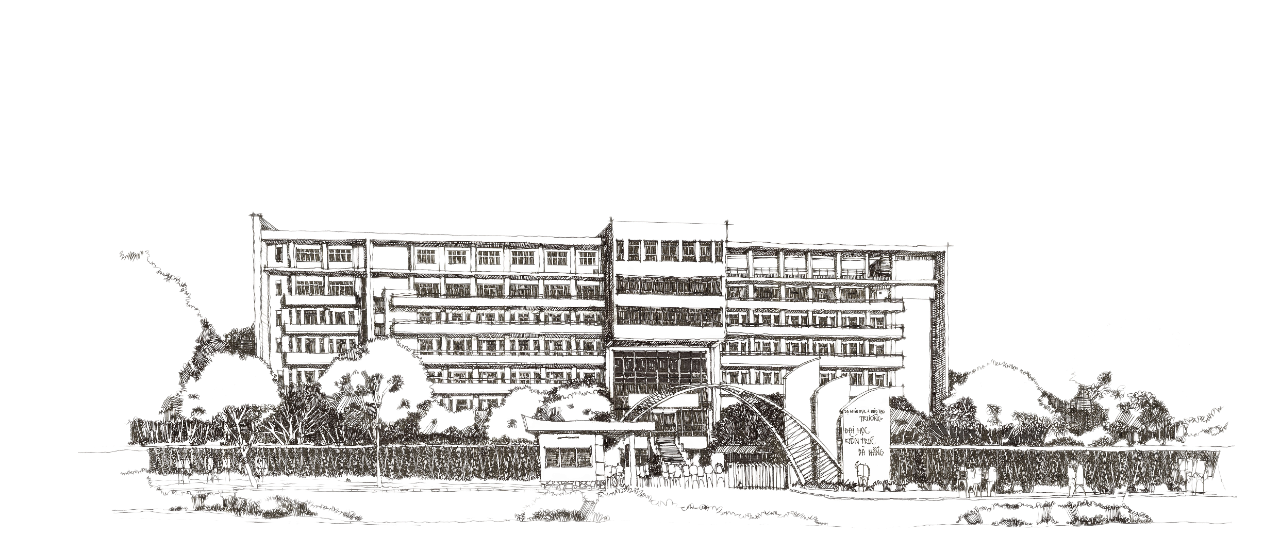
\includegraphics[width=0.7\paperwidth]{dau-campus.png}};
  \node[anchor=north west] at ([xshift=0.55cm, yshift=-0.45cm]current page.north west){
\includegraphics[height=0.9cm]{dau-logo.png}};
  \node[anchor=base, text=daumaroon] at ([yshift=-3.3cm]current page.north){\fontsize{52}{52}\selectfont\bfseries #1};
  \fill[daumaroon] ([yshift=-3.7cm]current page.north west) rectangle ([yshift=-5.15cm]current page.north east);
  \fill[daugold]   ([yshift=-5.15cm]current page.north west) rectangle ([yshift=-5.27cm]current page.north east);
  \node[anchor=center, text=white, align=center, text width=0.9\paperwidth] at ([yshift=-4.42cm]current page.north){\Large\bfseries #2};
\end{tikzpicture}
\end{frame}}}

% ---------- Metadata --------------------------------------------------
\title[Luồng KĐCLGD \, $\cdot$ \, kdcl-v2]{Hệ thống quản lý minh chứng KĐCLGD}
\subtitle{Mô tả luồng nghiệp vụ: đánh giá cơ sở giáo dục và minh chứng chương trình đào tạo}
\author{TS. Đỗ Phúc Hảo, Giám đốc Trung tâm CAIRA}
\institute{Trung tâm CAIRA, Trường Đại học Kiến trúc Đà Nẵng}
\date{\today}

% ---------- Macro khung demo: 1 ảnh lớn + chú thích ----------
\newcommand{\demoframe}[3]{%
\begin{frame}{#1}
\vspace{0.1cm}
\centering
\setlength{\fboxsep}{0pt}\setlength{\fboxrule}{0.6pt}%
\fcolorbox{gray300}{white}{\includegraphics[height=5.55cm]{#2}}\\[0.18cm]
\begin{minipage}{0.95\textwidth}\centering\footnotesize\color{charcoal}#3\end{minipage}
\end{frame}}

\title[Demo KĐCLGD \, $\cdot$ \, kdcl-v2]{Hệ thống quản lý minh chứng KĐCLGD}
\subtitle{Demo màn hình phần mềm theo luồng nghiệp vụ}

\begin{document}

% ============================ COVER ===================================
{\setbeamertemplate{headline}{}\setbeamertemplate{footline}{}
\begin{frame}[plain]
\begin{tikzpicture}[remember picture, overlay]
  \fill[daunavy] (current page.north west) rectangle (current page.south east);
  \node[anchor=south east, opacity=0.10] at ([xshift=-0.2cm,yshift=0.1cm]current page.south east){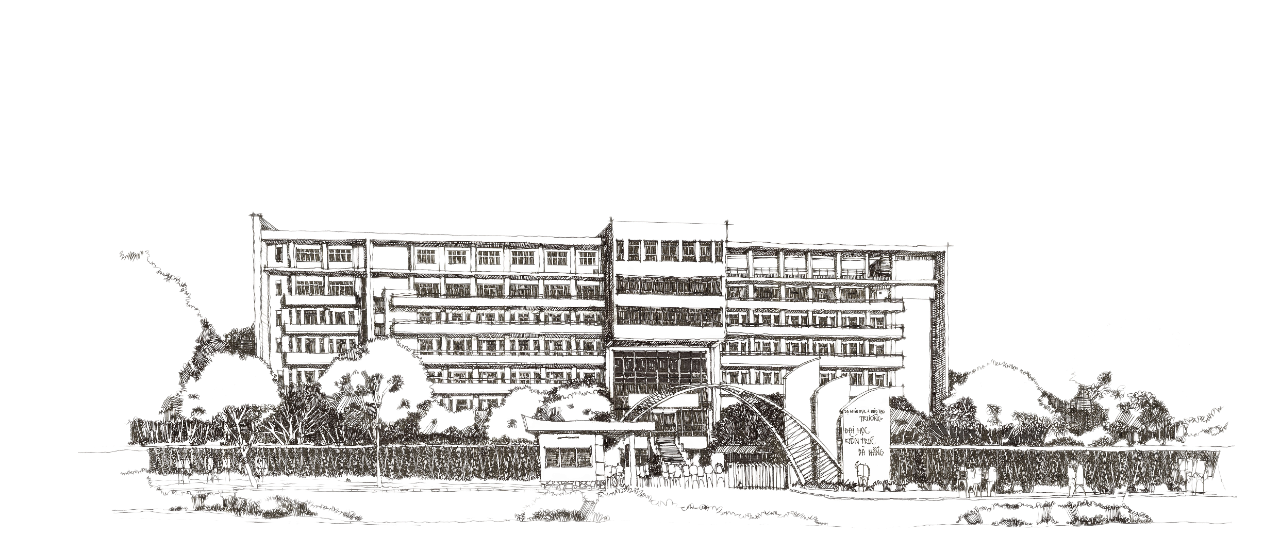
\includegraphics[width=0.52\paperwidth]{dau-campus.png}};
  \fill[daumaroon] ([yshift=-7.05cm]current page.north west) rectangle ([yshift=-7.25cm]current page.north east);
  \fill[daugold]   ([yshift=-7.25cm]current page.north west) rectangle ([yshift=-7.37cm]current page.north east);
  \node[anchor=north west] at ([xshift=0.6cm, yshift=-0.55cm]current page.north west){
\includegraphics[height=1.0cm]{dau-logo.png}};
  \node[anchor=north west, text width=13.6cm, inner sep=0, align=left] at ([xshift=0.6cm, yshift=-2.0cm]current page.north west){%
    \color{white}\raggedright
    {\normalsize\bfseries TRUNG TÂM CAIRA \, $\cdot$ \, TRƯỜNG ĐẠI HỌC KIẾN TRÚC ĐÀ NẴNG}\\[0.5cm]
    {\fontsize{24}{28}\selectfont\bfseries Hệ thống quản lý minh chứng KĐCLGD}\\[0.2cm]
    {\large\color{daugold}\bfseries Demo màn hình phần mềm theo luồng nghiệp vụ}\\[0.7cm]
    {\small\bfseries Trình bày:} {\small TS. Đỗ Phúc Hảo, Giám đốc Trung tâm CAIRA}\\[0.12cm]
    {\footnotesize\itshape Ảnh chụp thực tế từ phần mềm đang vận hành \, $\cdot$ \, dữ liệu mẫu}%
  };
  \node[anchor=north west, text width=13.6cm, inner sep=0, align=left] at ([xshift=0.6cm, yshift=-7.6cm]current page.north west){%
    \color{white!85}\raggedright {\small \today \, $\cdot$ \, Đà Nẵng}};
\end{tikzpicture}
\end{frame}}

% #####################################################################
\section{Đăng nhập và minh chứng}
\dividerframe{01}{Đăng nhập\\[2pt] và quản lý minh chứng}

\demoframe{Đăng nhập theo vai}{shots/01-login.png}{%
Đăng nhập bằng tài khoản theo vai: \textbf{admin} (P.ĐBCL), \textbf{đơn vị} (phòng/khoa), \textbf{lãnh đạo/đoàn}. Mật khẩu được băm, phiên đăng nhập qua cookie; mọi thao tác đều lưu dấu vết người thực hiện.}

\demoframe{Quản lý minh chứng}{shots/10-minhchung.png}{%
Cây \textbf{15 tiêu chuẩn / 60 tiêu chí} bên trái với số minh chứng từng tiêu chuẩn; bảng minh chứng mã hoá \texttt{Hn.ab.cd.ef}, hỗ trợ cả \textbf{tệp tải lên} và \textbf{liên kết Drive} (biểu tượng khóa liên kết).}

% #####################################################################
\section{Nộp - duyệt minh chứng}
\dividerframe{02}{Quy trình\\[2pt] nộp - duyệt minh chứng}

\demoframe{Cổng đơn vị}{shots/11-congdonvi.png}{%
Mỗi phòng/khoa thấy đúng các tiêu chí được giao, trạng thái từng minh chứng (\textbf{đủ / chờ duyệt / bị trả lại kèm lý do}) và nút tải minh chứng lên.}

\demoframe{Bàn duyệt của P.ĐBCL}{shots/12-banduyet.png}{%
Hàng đợi minh chứng các đơn vị vừa nộp. P.ĐBCL \textbf{xác nhận} nếu đạt, hoặc \textbf{trả lại kèm lý do} để đơn vị bổ sung.}

\demoframe{Đối soát theo tiêu chí}{shots/13-doisoat.png}{%
Màn hình cho Hội đồng và đoàn kiểm tra: mỗi tiêu chí hiển thị số minh chứng \textbf{đã xác nhận}, đơn vị phụ trách và cờ đủ/thiếu.}

\demoframe{Dashboard nộp - duyệt}{shots/14-dashduyet.png}{%
Tiến độ nộp và duyệt theo từng \textbf{đơn vị}, cùng \textbf{độ phủ} minh chứng theo tiêu chí, giúp biết còn thiếu chỗ nào trước khi đón đoàn.}

% #####################################################################
\section{Đánh giá, KPI, khảo sát, báo cáo}
\dividerframe{03}{Đánh giá, KPI,\\[2pt] khảo sát và báo cáo}

\demoframe{Đánh giá tiêu chí (Biểu 04)}{shots/15-danhgia.png}{%
Mỗi tiêu chí: hiện trạng, điểm mạnh, tồn tại, kế hoạch cải tiến; kết quả \textbf{Đạt / Không đạt}; trạng thái nháp hay đã duyệt.}

\demoframe{KPI - Biểu 16}{shots/16-kpi.png}{%
Số liệu theo \textbf{năm học} với biểu đồ xu hướng: tỉ lệ tốt nghiệp, việc làm, mức độ hài lòng và số công bố khoa học.}

\demoframe{Tiến độ tự đánh giá}{shots/17-tiendo.png}{%
Kế hoạch \textbf{24 tuần / 5 giai đoạn}; theo dõi trạng thái từng công việc (hoàn thành / đang làm / trễ hạn).}

\demoframe{Khảo sát các bên (Biểu 08-11)}{shots/18-khaosat.png}{%
Tạo phiếu khảo sát cán bộ, người học, nhà tuyển dụng, cựu sinh viên; phát \textbf{liên kết công khai} theo mã và tự tổng hợp kết quả.}

\demoframe{Báo cáo tự đánh giá (Biểu 05)}{shots/19-baocao.png}{%
Tổng hợp cơ sở pháp lý, quá trình tự đánh giá, kết quả 15 tiêu chuẩn và kế hoạch cải tiến.}

\demoframe{Dashboard lãnh đạo}{shots/20-dashboard.png}{%
Nhìn nhanh toàn cảnh: radar 15 tiêu chuẩn, xu hướng KPI theo năm và tổng hợp khảo sát các bên.}

% #####################################################################
\section{Chương trình đào tạo (Kiến trúc)}
\dividerframe{04}{Chương trình đào tạo\\[2pt] ngành Kiến trúc}

\demoframe{Tổng quan chương trình đào tạo}{shots/30-ctdt.png}{%
Đợt kiểm định chương trình đào tạo \textbf{ngành Kiến trúc}: trạng thái khung chuẩn đầu ra và tiến độ đo lường.}

\demoframe{Khung chuẩn đầu ra}{shots/31-cdr.png}{%
Khai báo \textbf{PEO - PLO - CLO}: mục tiêu giáo dục, chuẩn đầu ra chương trình và chuẩn đầu ra từng học phần.}

\demoframe{Ma trận ánh xạ}{shots/32-matran.png}{%
Ánh xạ \textbf{học phần lên PLO} theo mức I/R/M và \textbf{CLO lên PLO} theo trọng số, cho thấy chương trình phủ đủ chuẩn đầu ra.}

\demoframe{Thư viện Rubric}{shots/33-rubric.png}{%
Bộ \textbf{rubric} thang đánh giá chuẩn đầu ra, dùng để chấm đồ án và các bài đánh giá của học phần.}

\demoframe{Đo lường CLO}{shots/34-doclo.png}{%
Nhập điểm theo từng bài đánh giá; hệ thống tự tính \textbf{tỉ lệ đạt từng CLO} theo trọng số.}

\demoframe{Tổng hợp PLO (AUN-QA)}{shots/35-plo.png}{%
Cuộn kết quả CLO lên \textbf{PLO}, phân loại theo \textbf{4 mức AUN-QA}. Ngành Kiến trúc đạt \textbf{100\%} ở các PLO đã đo (mức đạt hoàn toàn).}

% ---- Cảm ơn ----
{\setbeamertemplate{headline}{}\setbeamertemplate{footline}{}
\begin{frame}[plain]
\begin{tikzpicture}[remember picture, overlay]
  \fill[daunavy] (current page.north west) rectangle (current page.south east);
  \node[anchor=south east, opacity=0.10] at ([xshift=-0.2cm,yshift=0.1cm]current page.south east){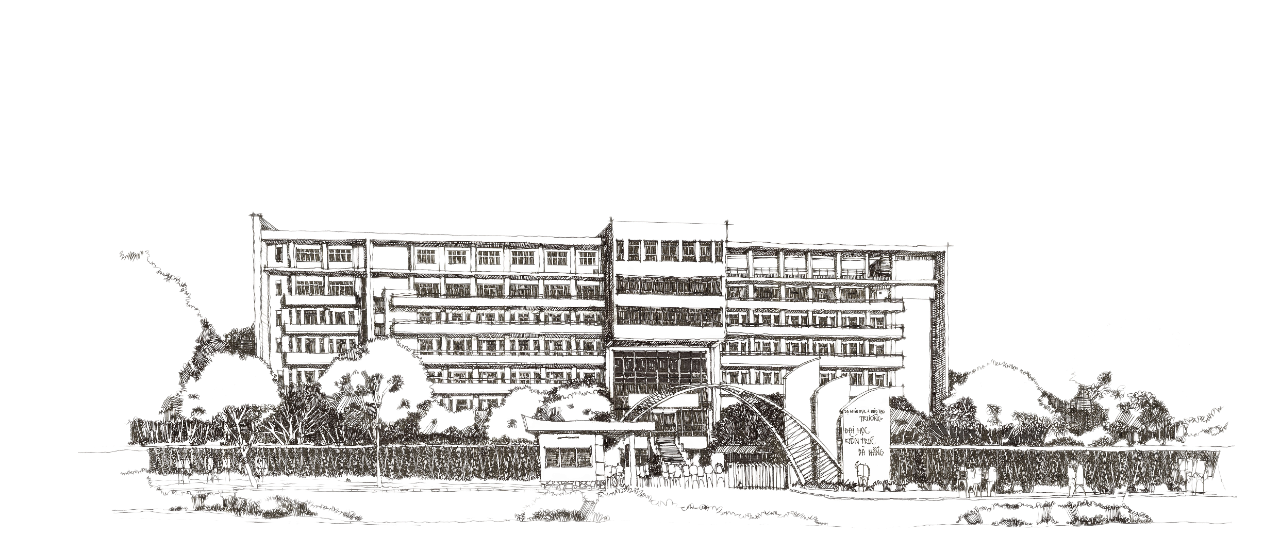
\includegraphics[width=0.5\paperwidth]{dau-campus.png}};
  \node[anchor=north west] at ([xshift=0.6cm, yshift=-0.6cm]current page.north west){
\includegraphics[height=1.0cm]{dau-logo.png}};
  \fill[daumaroon] ([yshift=-4.4cm]current page.north west) rectangle ([yshift=-4.6cm]current page.north east);
  \fill[daugold]   ([yshift=-4.6cm]current page.north west) rectangle ([yshift=-4.72cm]current page.north east);
  \node[anchor=center, text=white, align=center, text width=0.9\paperwidth] at ([yshift=-3.3cm]current page.north){\fontsize{34}{38}\selectfont\bfseries Trân trọng cảm ơn};
  \node[anchor=center, text=white!85, align=center, text width=0.9\paperwidth] at ([yshift=-5.5cm]current page.north){%
    \normalsize TS. Đỗ Phúc Hảo \, $\cdot$ \, Giám đốc Trung tâm CAIRA\\[4pt]
    \small Trường Đại học Kiến trúc Đà Nẵng};
\end{tikzpicture}
\end{frame}}

\end{document}
